\documentclass[11pt]{article}
\usepackage[a4paper,left=20mm,top=10mm,bottom=10mm]{geometry}
\usepackage[OT2]{fontenc}
\pagenumbering{gobble}
\usepackage{amsfonts}
\usepackage{graphicx}
\usepackage{amsthm}
\newcommand\tsd{\theoremstyle{definition}}
\newcommand\tsr{\theoremstyle{remark}}
\newcommand\D{\displaystyle}
\setlength{\parindent}{0pt}

\tsd\newtheorem{zad}{Zadatak}
\newcommand\eng{\fontencoding{OT1}\fontfamily{\rmdefault}\selectfont}
\newcommand\srb{\fontencoding{OT2}\fontfamily{\rmdefault}\selectfont}

\title{\bf{Vezhbe iz fizike}}
\author{\Large Aleksa Vuchkovic1, 3c}
\date{}

\begin{document}
\maketitle
\large

\textbf{\Large Vezhba 3. Omov zakon za celo strujno kolo}\\
\textit{Odredjivanje elektromotorne sile i unutrashnjeg otpora izvora jednosmerne struje}\\

\addtolength{\tabcolsep}{5pt}
\begin{tabular}{|c@{\hspace{10pt}} *{5}{|c}}
\hline
Broj Merenja & $I [ 10^{-3} A ]$ & $\Delta I[ 10^{-3} A ]$ & $U[10^{-2}V]$ & $\Delta U[10^{-2}V]$ \\ [1ex]
\hline
1 & 25,3 & 0,5 & 143,0  & 1,1\\
\hline
2 & 30,2  & 0,5  & 142,3 & 1,1\\
\hline
3  & 34,9 & 0,5 & 141,6 & 1,1\\
\hline
4 & 40,0 & 0,5 & 140,8 & 1,1\\
\hline
5 & 45,0 & 0,6 & 140,0 & 1,1\\
\hline
6 & 49,9 & 0,6 & 139,4 & 1,1\\
\hline
7 & 55,3 & 0,6 & 138,5 & 1,1\\
\hline
8 & 59,9 & 0,6 & 137,8 & 1,1\\
\hline
9 & 65,2 & 0,7 & 137,0 & 1,1\\
\hline
\end{tabular}\\[5mm]
Crtamo grafik zavisnosti $U=f(I)$, gde je koeficijent prave jednak $-r$, a presek sa ordinatom je  $\epsilon$.\\
$U = -rI + \epsilon$\\
$k$ - koeficijent pravca prave\\\\
$A = (28 \cdot 10^{-3} A, 142.6 \cdot 10^{-2} V)$\\
$B = (62 \cdot 10^{-3} A, 137.5 \cdot 10^{-2} V)$\\

$k=\D\frac{U_b - U_a}{I_b - I_a} = \D\frac{-5.1 \cdot 10^{-2} V}{34 \cdot 10^{-3}A} = -1.5\Omega$\\[3mm]
$\delta_k = \D\frac{\Delta U_b + \Delta U_a}{|U_b - U_a|} + \D\frac{\Delta I_b + \Delta I_a}{|I_b - I_a|} = \frac{1.1 \cdot 10^{-2}V + 1.1\cdot 10^{-2}V}{5.1 \cdot 10^{-2}V} + \D\frac{0.7\cdot 10^{-3}A + 0.5\cdot 10^{-3}A}{34 \cdot 10^{-3}A} =\\= \D\frac{2.2}{5.1} + \D\frac{1.2}{34} = 0.4666$\\[8mm]
$\Delta k =\delta_k \cdot k = 0.4666 \cdot (-1.5\Omega) = -0,6999\Omega \approx -0.7\Omega$\\
$(k \pm \Delta k) = -(1.5 \pm 0.7)\Omega = -r$\\[5mm]
$r = (1.5 \pm 0.7)\Omega$\\[5mm]
Odredili smo otpor izvora, sad nam preostaje josh elektromotorna sila,\\ koju dobijamo iz preseka prave sa $y$-osom...\\

Sa grafika mozhemo prochitati vrednost elektromotorne sile,\\
gde je $\Delta\epsilon=\Delta U_{max}.$\\[5mm]
$(\epsilon\pm\Delta\epsilon)=(146.8\pm 1.1)\cdot10^{-2}V$\\

Grafik na milimetarskom papiru se mozhe videti na sledec1oj strani dokumenta.
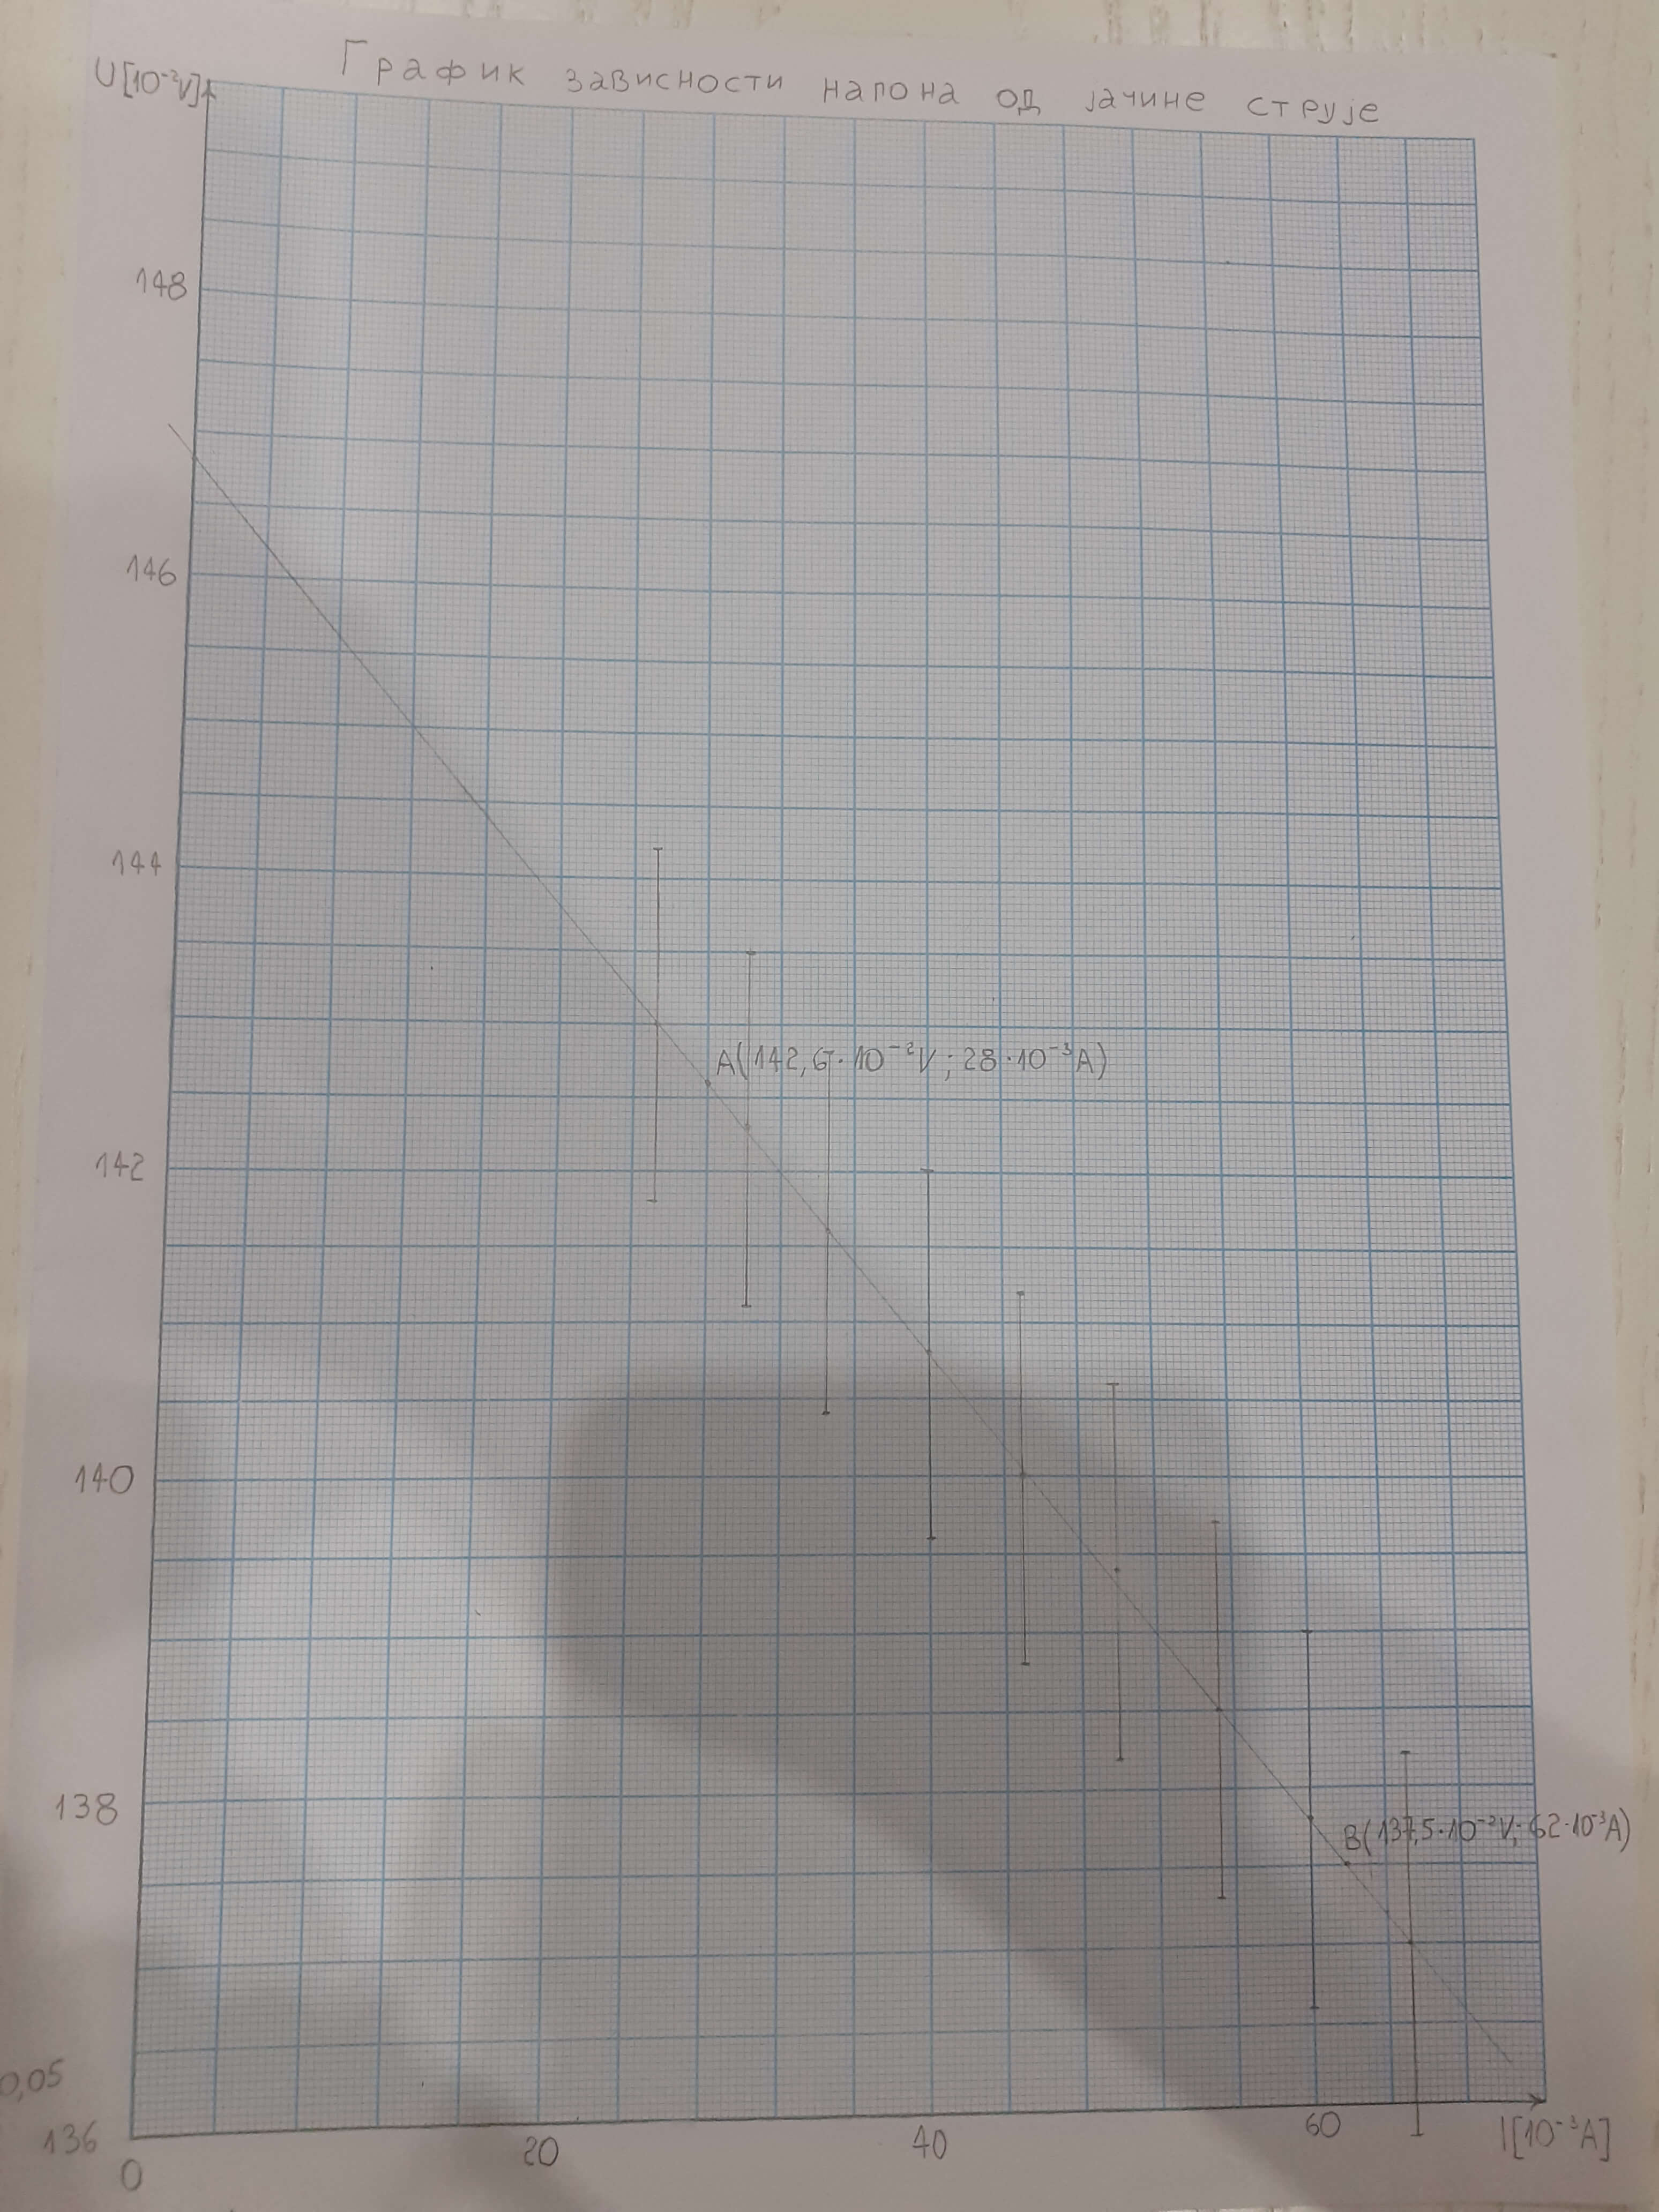
\includegraphics[scale=0.16]{slika.jpg}
\end{document}